\documentclass[10pt, compress, aspectratio=169]{beamer}

\usetheme[numbering=fraction, progressbar=none, titleformat=smallcaps, sectionpage=none]{metropolis}

\usepackage{sourcecodepro}
\usepackage{booktabs}
\usepackage{array}
\usepackage{listings}
\usepackage{graphicx}
\usepackage[english]{babel}
\usepackage[scale=2]{ccicons}
\usepackage{url}
\usepackage{relsize}
\usepackage{wasysym}

\usepackage{pgfplots}
\usepgfplotslibrary{dateplot}

\definecolor{Base}{HTML}{191F26}
\definecolor{Accent}{HTML}{157FFF}

\setbeamercolor{alerted text}{fg=Accent}
\setbeamercolor{frametitle}{bg=Base}

\setsansfont[BoldFont={Source Sans Pro Semibold},
              Numbers={OldStyle}]{Source Sans Pro}

\lstset{ %
  backgroundcolor={},
  basicstyle=\ttfamily\footnotesize,
  breakatwhitespace=true,
  breaklines=true,
  captionpos=n,
  commentstyle=\color{orange},
  escapeinside={\%*}{*)},
  extendedchars=true,
  frame=n,
  keywordstyle=\color{Accent},
  language=C++,
  rulecolor=\color{black},
  showspaces=false,
  showstringspaces=false,
  showtabs=false,
  stepnumber=2,
  stringstyle=\color{gray},
  tabsize=2,
  keywords={thrust,plus,device_vector, copy,transform,begin,end, copyin,
  copyout, acc, \_\_global\_\_, void, int, float, main, threadIdx, blockIdx,
  blockDim, if, else, malloc, NULL, cudaMalloc, cudaMemcpy, cudaSuccess,
  cudaGetLastError, cudaDeviceSynchronize, cudaFree, cudaMemcpyDeviceToHost,
  cudaMemcpyHostToDevice, const, data, independent, kernels, loop,
  fprintf, stderr, cudaGetErrorString, EXIT_FAILURE, for, dim3},
  otherkeywords={::, \#pragma, \#include, <<<,>>>, \&, \*, +, -, /, [, ], >, <}
}

\renewcommand*{\UrlFont}{\ttfamily\smaller\relax}

\graphicspath{{../img/}}

\title{Title Goes Here}
\author{\footnotesize Pedro Bruel \\ {\scriptsize \emph{phrb@ime.usp.br}}}
\institute{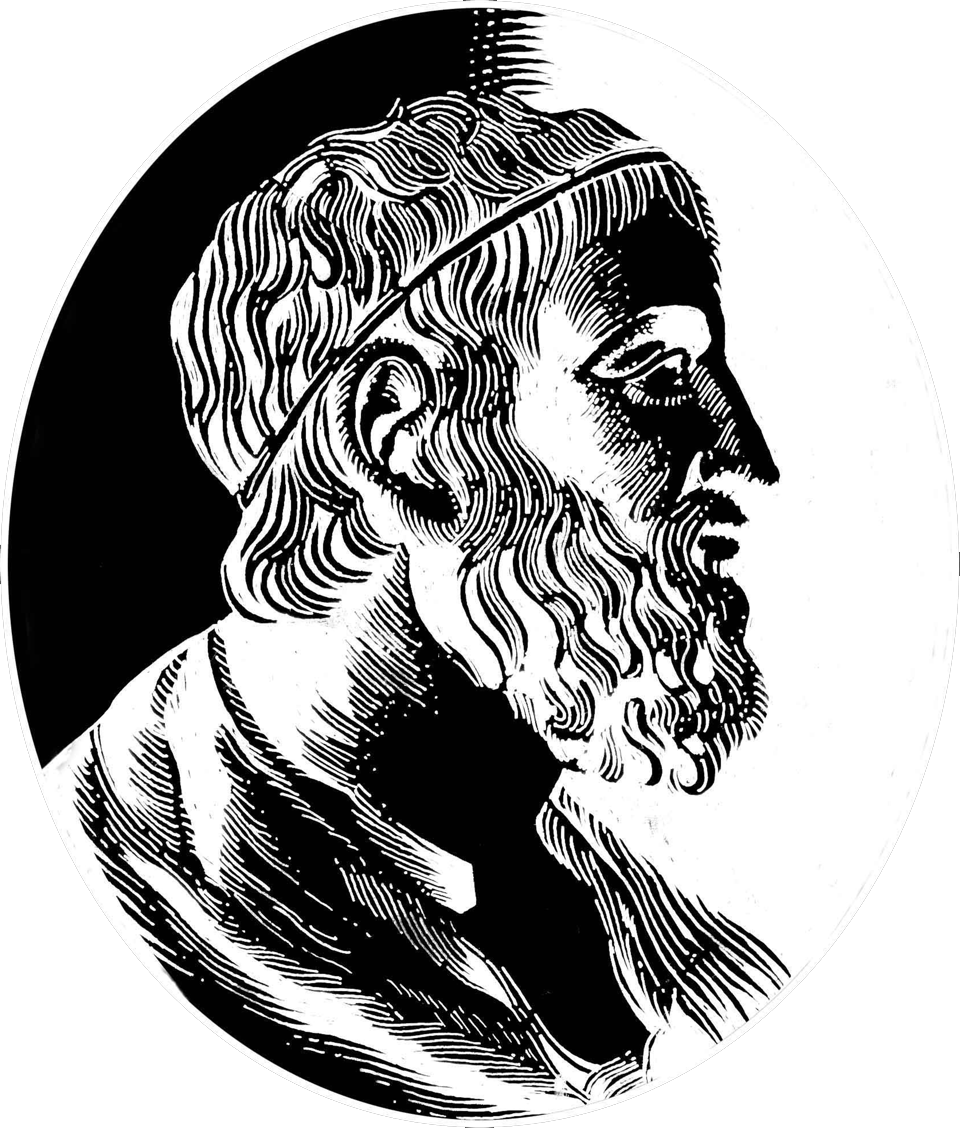
\includegraphics[height=2cm]{imelogo}\\[0.2cm] Instituto de Matemática e Estatística \\ Universidade de São Paulo}
\date{\scriptsize \today}

\begin{document}

\maketitle

\part{Part I}

\section{Introduction}

\subsection{About}

\begin{frame}
    \frametitle{About}
    \begin{columns}[T,onlytextwidth]
        \column{0.5\textwidth}
        \begin{center}
            
\includegraphics[width=.45\textwidth]{pedro}

            Pedro Bruel \\
            \emph{\alert{phrb}@ime.usp.br} \\[.3cm]
            \url{www.ime.usp.br/~phrb} \\
            \url{github.com/phrb} \\
        \end{center}

        \column{0.5\textwidth}
        \begin{center}
            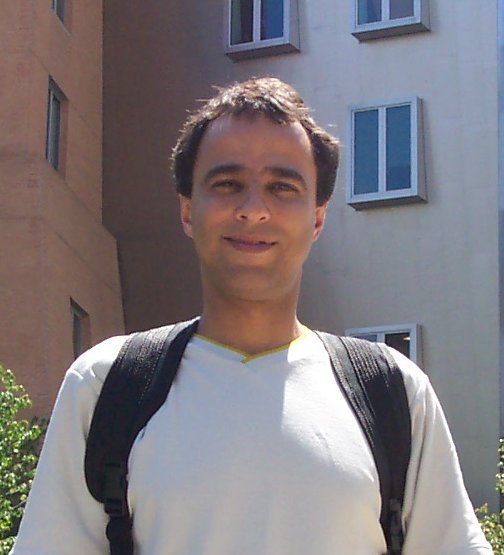
\includegraphics[width=.4\textwidth]{alfredo}

            Alfredo Goldman \\
            \emph{\alert{gold}@ime.usp.br} \\[.3cm]
            \url{www.ime.usp.br/~gold} \\
        \end{center}
    \end{columns}
\end{frame}

\subsection{Index}

\begin{frame}
    \frametitle{Index}
    \setbeamertemplate{section in toc}[sections numbered]
    \tableofcontents[hideallsubsections, part=1]
\end{frame}

\begin{frame}
    \frametitle{Slides}
    \begin{center}
        
\includegraphics[width=.18\textwidth]{github}
    \end{center}
    The slides and all source code are hosted at \alert{GitHub}:

    \begin{itemize}
        \item \url{github.com/phrb/---}
    \end{itemize}
\end{frame}

\begin{frame}[fragile]
    \frametitle{Sample Code}
    \begin{lstlisting}[basicstyle=\ttfamily\scriptsize]
    #include <cuda_runtime.h>

    float *h_A = (float *) malloc(size);
    if (h_A == NULL) { ... };

    float *d_A = NULL;
    err = cudaMalloc((void **) &d_A, size);
    err = cudaMemcpy(d_A, h_A, size, cudaMemcpyHostToDevice);
    if (err != cudaSuccess) { ... };

    int threadsPerBlock = 256;
    int blocksPerGrid = (numElements + threadsPerBlock - 1) / threadsPerBlock;

    vectorAdd<<<blocksPerGrid, threadsPerBlock>>>(d_A, d_B, d_C, numElements);

    err = cudaGetLastError();
    err = cudaDeviceSynchronize();
    if (err != cudaSuccess) { ... };

    err = cudaMemcpy(h_C, d_C, size, cudaMemcpyDeviceToHost);
    err = cudaFree(d_A);
    if (err != cudaSuccess) { ... };
    \end{lstlisting}

    \vfill

    \begin{center}
        \tiny{Fonte: \url{github.com/phrb/intro-cuda} [Accessed in 29/07/16]}
    \end{center}
\end{frame}

\maketitle

\end{document}
